% !TeX root = ../main.tex
\appendix

\chapter{Installation Manual}
\label{app:installation_manual}

This appendix is the procedure for running the prototype on a single machine. The commands are issued from the root of the repository. The stack is the one started by Docker Compose: the simulator, the broker, the streaming jobs, the lakehouse, the time-series store, the dashboards, and the three utilities. Training is a separate step and does not start with the rest.

\section{Prerequisites}

The host needs Git and Docker Engine with the Compose plugin (\texttt{docker compose}, not the older \texttt{docker-compose} binary). A Linux host is the path used during development. The same Compose file runs under Docker Desktop on Windows through WSL2. The first start builds several images, so the machine needs a few gigabytes free for images and for the MinIO and Redpanda volumes. No GPU is required for the stack itself. A GPU is used only when a training run is launched outside the CPU image.

\section{Configuration}

Clone the repository and enter its root. Copy the example environment file if a local one does not exist yet:

\begin{lstlisting}[basicstyle=\ttfamily\small,breaklines=true]
cp .env.example .env
\end{lstlisting}

\texttt{.env.example} is the contract of host ports, topic names, and credentials. The development defaults are the ones used below (\texttt{admin} / \texttt{admin} for Grafana, \texttt{admin} / \texttt{admin123456} for MinIO). Change them in \texttt{.env} before any deployment that is not a local demonstration. Do not commit \texttt{.env}.

\section{Starting the platform}

From the repository root:

\begin{lstlisting}[basicstyle=\ttfamily\small,breaklines=true]
docker compose up -d --build
\end{lstlisting}

Compose builds the local images (the simulator, the orchestrator, the digital twin, the portal, and the inference job) and pulls the others. The first start is the slow one. Later starts reuse the images. When the command returns, open the platform portal at \texttt{http://localhost:8080}. A service that is still starting shows as down for a short time. Refresh until the broker, Redpanda, MinIO, QuestDB, Grafana, MLflow, the orchestrator, and the twin answer. The one-shot containers that create the bucket, the topics, and the QuestDB tables exit on their own. That is expected.

The factory anchors the five vehicles and then runs without further commands. Telemetry reaches Grafana after the Silver job has published \texttt{fleet-features} and Kafka Connect has written QuestDB. Anomaly scores appear only after a model version carries the \texttt{production} alias, as described in the user manual.

\section{Training run}

Training is the Compose profile \texttt{ml}. It is not part of \texttt{docker compose up}. MinIO and MLflow must already be healthy. The run name is built from the capture label, so pass \texttt{--dataset-id}. Dates are UTC.

\begin{lstlisting}[basicstyle=\ttfamily\small,breaklines=true]
docker compose --profile ml run --rm ml-train \
  --dataset-id factory-2026-11-20 \
  --start-date 2026-11-20T19:40:00Z \
  --end-date 2026-11-23T07:50:21Z
\end{lstlisting}

The experiment stays \texttt{agv-anomaly-detection} and the registered model stays \texttt{agv-gru-autoencoder}. Do not override those names for a run that should be comparable with the others. Windows with a gap above five seconds are dropped.

\section{Stopping}

\begin{lstlisting}[basicstyle=\ttfamily\small,breaklines=true]
docker compose down
\end{lstlisting}

This stops the containers and keeps the volumes: the lakehouse, QuestDB, the model registry, and the factory ledger remain. Adding \texttt{-v} deletes those volumes. Use it only when the stored telemetry and the registered models can be discarded.

\section{Exposed services}
\label{sec:service_ports_ui}

Table~\ref{tab:service_ports} lists the host ports. The web interfaces are the ones used in Appendix~\ref{app:user_manual}. The remaining ports are protocols.

\begin{table}[htbp]
\centering
\small
\caption{Host ports of the prototype.}
\label{tab:service_ports}
\begin{tabularx}{\linewidth}{@{}l l X@{}}
\toprule
\textbf{Service} & \textbf{Address} & \textbf{Role} \\
\midrule
Platform portal & \texttt{localhost:8080} & Health of the stack and links to every interface. \\
\addlinespace
Node-RED & \texttt{localhost:1880} & Factory flows. Fault console at \texttt{/ui/faults}. \\
\addlinespace
Digital twin & \texttt{localhost:8090} & Three-dimensional view of the factory. \\
\addlinespace
Grafana & \texttt{localhost:3000} & Dashboards. Login \texttt{admin} / \texttt{admin}. \\
\addlinespace
MLflow & \texttt{localhost:5000} & Experiments and the model registry. \\
\addlinespace
QuestDB console & \texttt{localhost:9000} & SQL over the time-series tables. \\
\addlinespace
MinIO console & \texttt{localhost:9001} & Buckets. Login \texttt{admin} / \texttt{admin123456}. \\
\addlinespace
Redpanda Console & \texttt{localhost:9080} & Topics \texttt{vda5050-state}, \texttt{fleet-features}, \texttt{ai-anomalies}. \\
\midrule
Mosquitto & \texttt{localhost:1883} & MQTT. WebSocket for the twin on \texttt{9883}. \\
\addlinespace
QuestDB wire & \texttt{localhost:8812} & Read by Grafana. User \texttt{grafana} / \texttt{grafana}. \\
\addlinespace
QuestDB ILP & \texttt{localhost:9009} & Ingestion port. Not a user interface. \\
\addlinespace
MinIO S3 API & \texttt{localhost:19000} & Object API, mapped from container port 9000. \\
\addlinespace
Redpanda & \texttt{localhost:19092} & Kafka protocol. Admin API on \texttt{19644}. \\
\addlinespace
Kafka Connect & \texttt{localhost:8083} & Connector status. \\
\bottomrule
\end{tabularx}
\end{table}

The simulator, Telegraf, and the Spark jobs (\texttt{spark-vda5050-state}, \texttt{spark-fleet-features}, \texttt{spark-anomaly-detector}, and \texttt{spark-maintenance}) have no host port. They are reached through the portal only as health checks.

\chapter{User Manual}
\label{app:user_manual}

The operator does not send orders by hand. The factory orchestrator dispatches missions, and the useful actions are to watch the plant, inject a fault, read the dashboards, and, when a new model has been trained, mark the version that inference should serve. Start from the portal. Every address in this appendix is on \texttt{localhost} and matches Table~\ref{tab:service_ports}.

\section{Opening the platform}

Open \texttt{http://localhost:8080}. The page lists each service, whether it answers, and how long the probe took. Use it as the index: Grafana, QuestDB, Redpanda Console, MinIO, MLflow, the orchestrator, and the twin are one click away. A red entry means that service is down. Fix that before looking for missing telemetry.

\begin{figure}[ht]
  \centering
  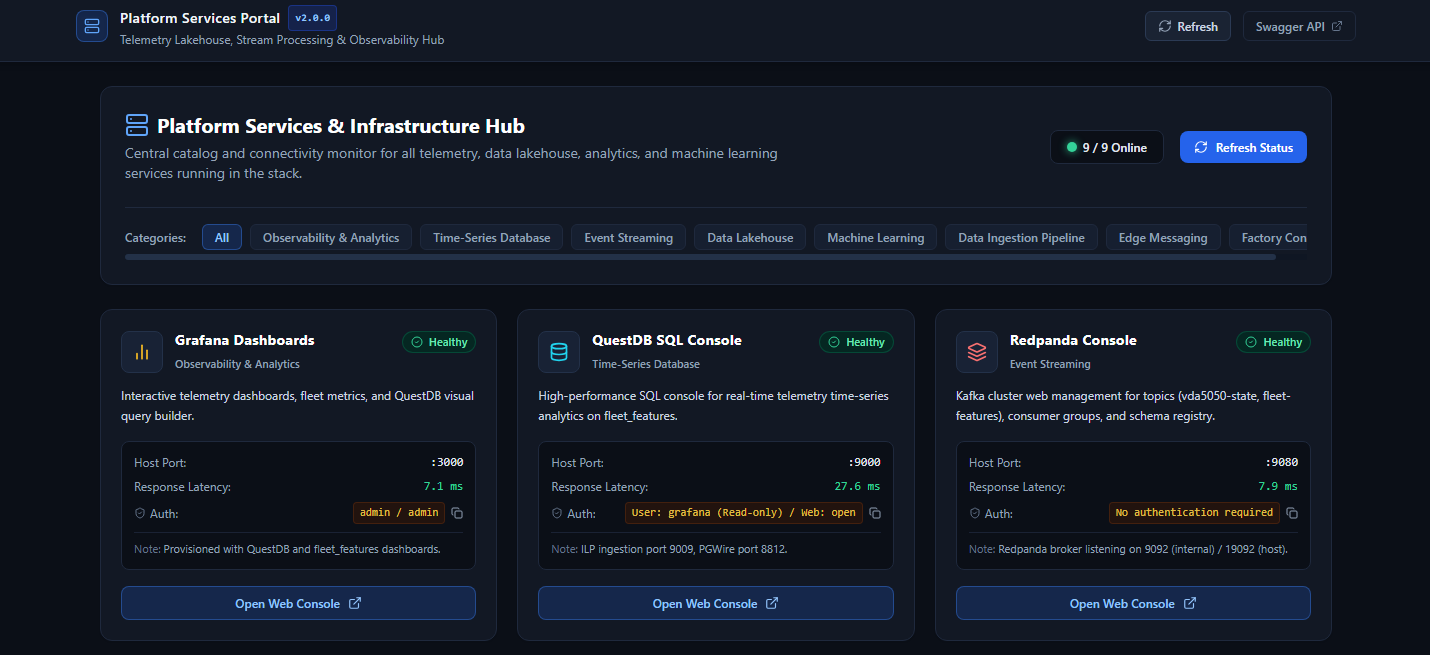
\includegraphics[width=0.95\linewidth]{openingThePlatform.png}
  \caption{Platform portal. Each service is listed with its health and a link to its interface.}
  \label{fig:manual-portal}
\end{figure}

\section{Watching the factory}

Open the digital twin at \texttt{http://localhost:8090}. Five vehicles move through the plant: wheels and chassis leave production, cross the warehouses, meet at assembly, and the finished good leaves for dispatch. A vehicle that is charging sits at its own dock. The page only subscribes. It does not accept orders.

\begin{figure}[ht]
  \centering
  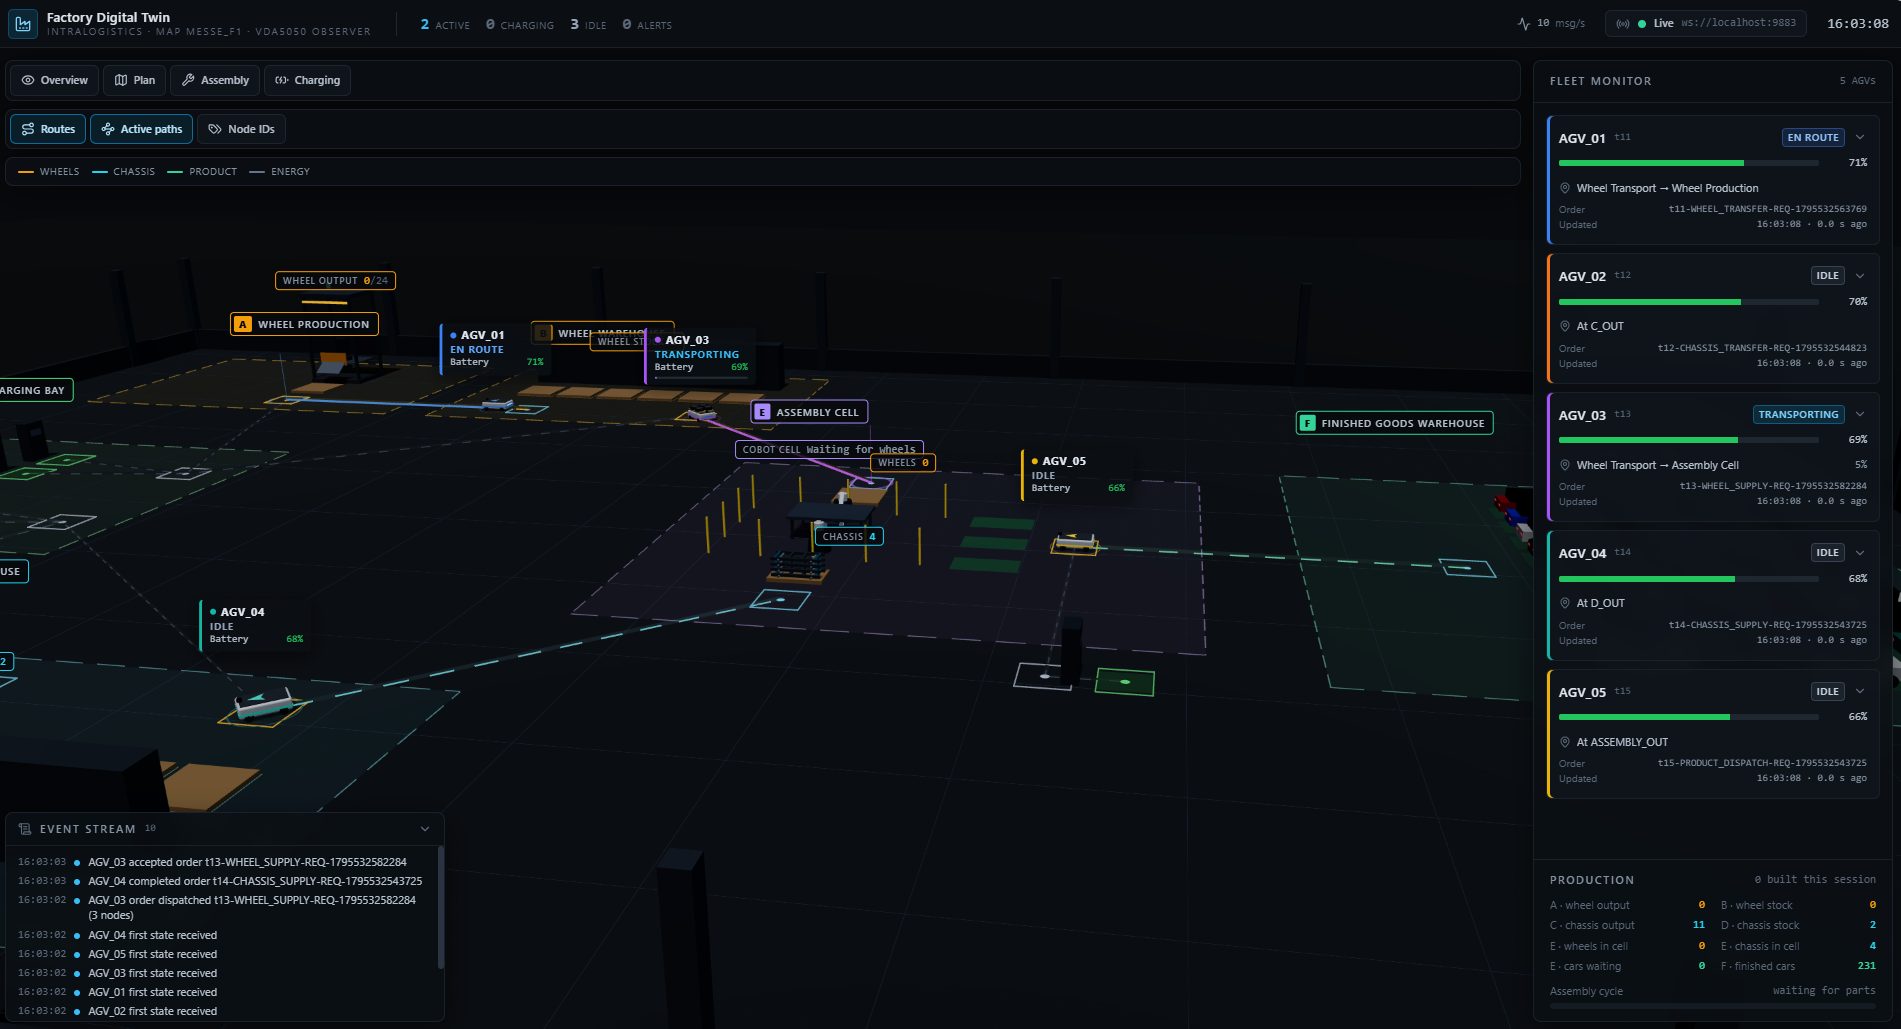
\includegraphics[width=0.95\linewidth]{WatchingTheFactory.png}
  \caption{Digital twin of the factory, with the five vehicles and the plant zones.}
  \label{fig:manual-twin}
\end{figure}

The same process is driven by Node-RED at \texttt{http://localhost:1880}. The editor shows the flows (configuration, bootstrap, state ingestion, order templates, production, the scheduler, and the fault console). The flow file is mounted read-only, so a deploy from the editor does not change the running factory. Restart the \texttt{factory-orchestrator} service after a change to the file in the repository.

\begin{figure}[ht]
  \centering
  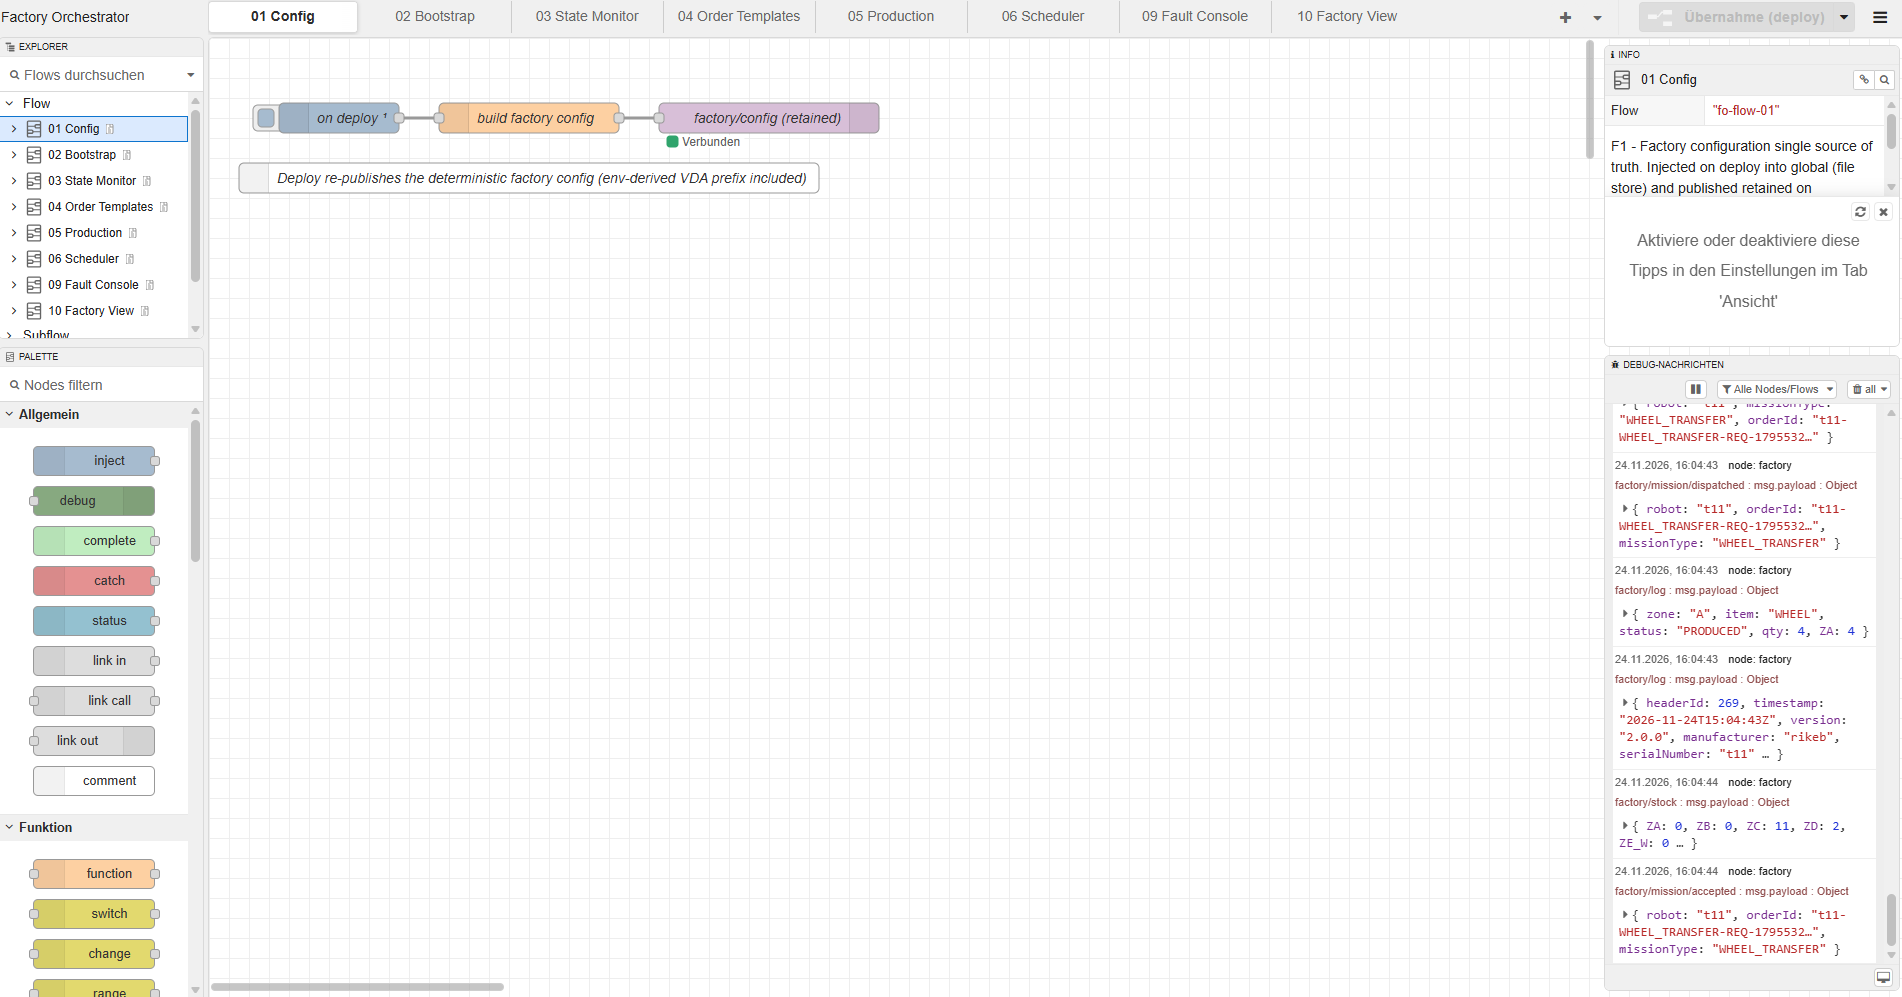
\includegraphics[width=0.95\linewidth]{watchingTheFactoryNodeRed.png}
  \caption{Node-RED editor with the factory flow tabs.}
  \label{fig:manual-nodered}
\end{figure}

\section{Injecting a fault}

Faults are applied from the dashboard at \texttt{http://localhost:1880/ui/faults}. Choose one vehicle, a fault type, and a severity, then inject. The severity is mapped to the intensity the simulator applies to the physics. Clearing the fault, or resetting faults, uses the same page. The missions do not change: the vehicle keeps the factory role, and the telemetry is what changes. The available faults are a mechanical stall, gearbox degradation, wheel wear, bearing degradation, a stator short circuit, and battery state-of-health degradation.

\begin{figure}[ht]
  \centering
  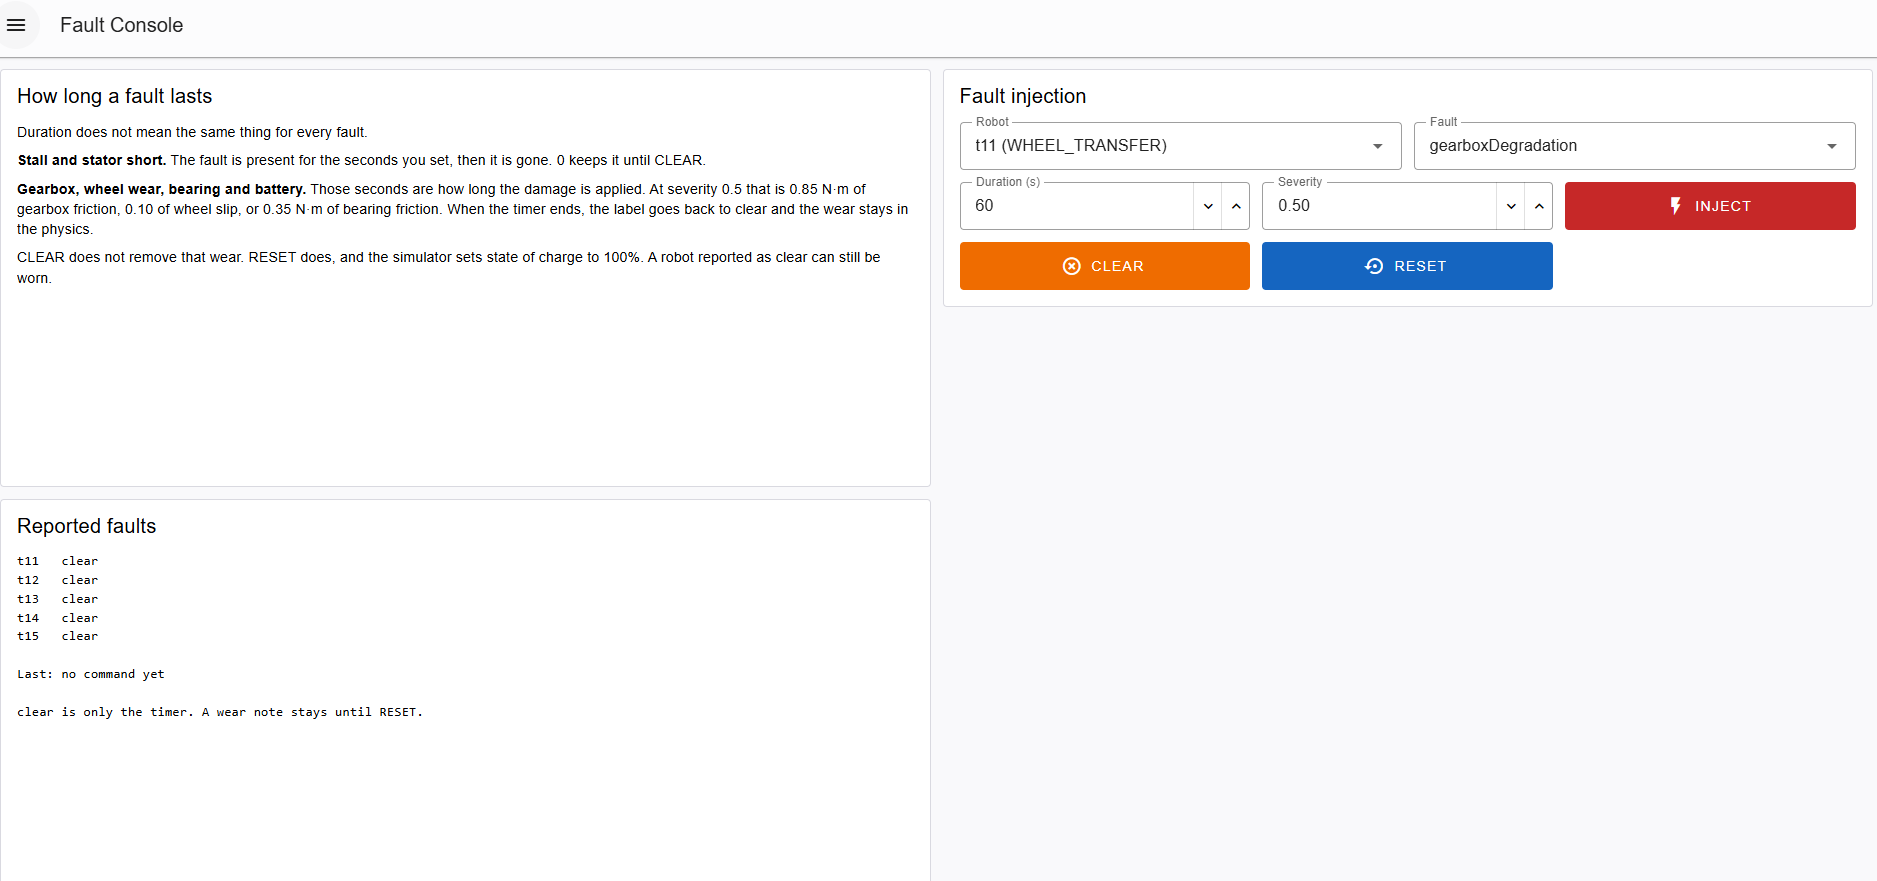
\includegraphics[width=0.95\linewidth]{injectAFault.png}
  \caption{Fault console. One vehicle, one fault type, and a severity.}
  \label{fig:manual-fault}
\end{figure}

After a few seconds the effect is visible on the powertrain dashboard (current, temperature, or voltage, depending on the fault) and, once a production model is loaded, on the anomaly dashboard.

\section{Reading the dashboards}

Grafana is at \texttt{http://localhost:3000}, with user \texttt{admin} and password \texttt{admin}. The dashboards are under the \texttt{questdb} folder. Each one refreshes every five seconds and can be filtered by vehicle.

\begin{itemize}
    \item \textbf{Fleet Battery.} State of charge, state of health, voltage, current, and temperature.
    \item \textbf{Fleet Velocity.} Linear velocity \(v_x\) and yaw rate \(\omega\).
    \item \textbf{Fleet Powertrain Physics.} The motor, thermal, and battery equations next to the measured channels.
    \item \textbf{Fleet Features --- Canonical Silver Overview.} The curated feature stream in one table.
    \item \textbf{AGV Anomaly Detection \& ML Inference.} Counts of normal, suspicious, and anomalous windows, the reconstruction score against the two thresholds, and the channels that dominate an elevated score.
\end{itemize}

\begin{figure}[ht]
  \centering
  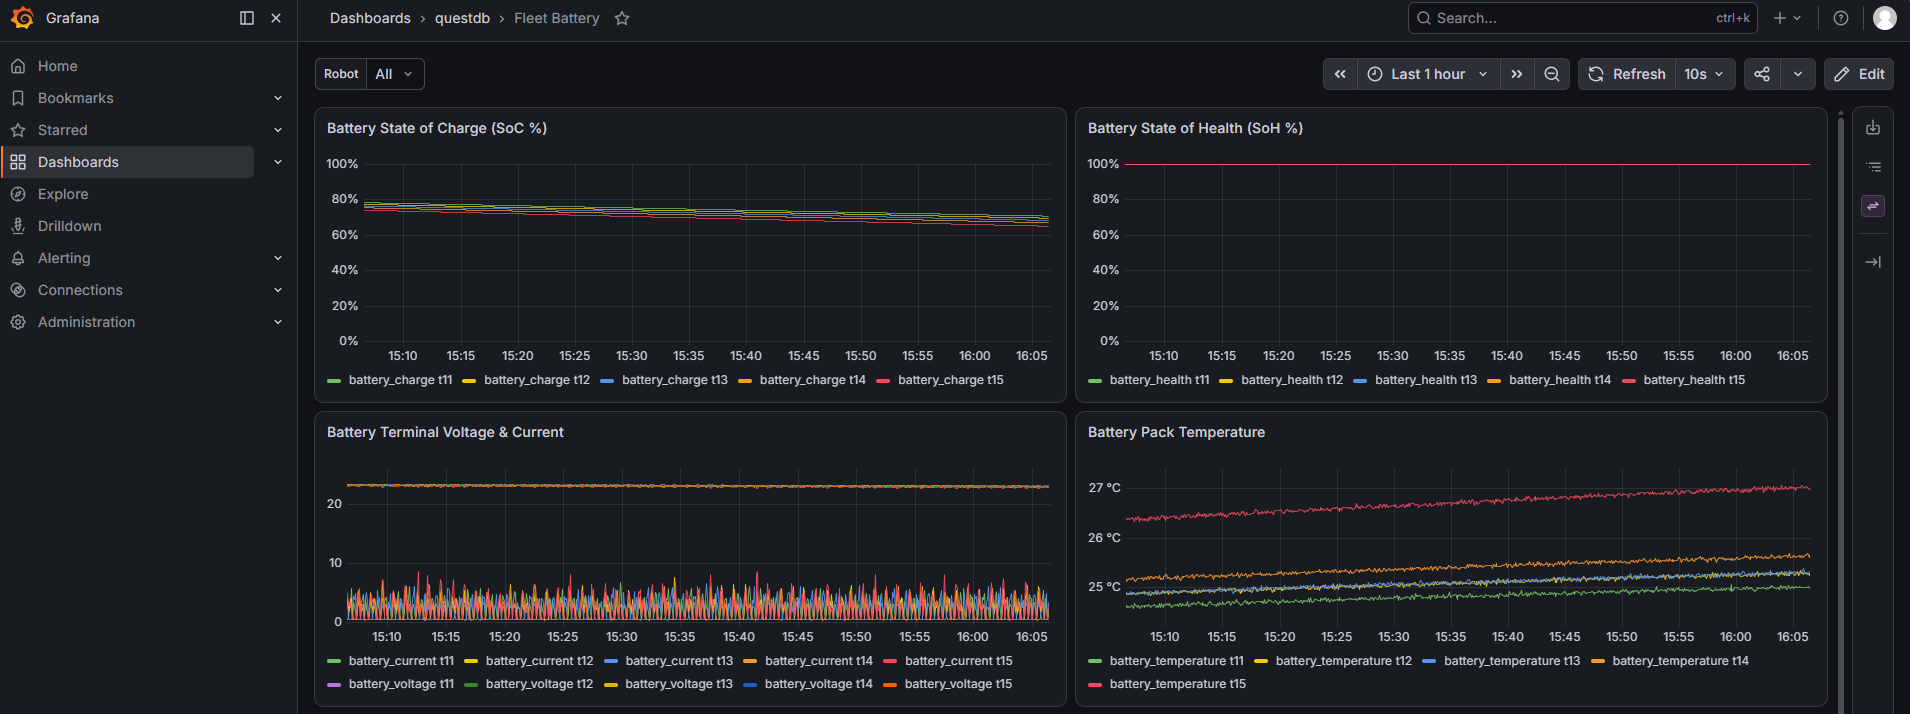
\includegraphics[width=0.95\linewidth]{grafanaFleetBatteryDashboard.png}
  \caption{Grafana Fleet Battery dashboard.}
  \label{fig:manual-grafana-battery}
\end{figure}

\begin{figure}[ht]
  \centering
  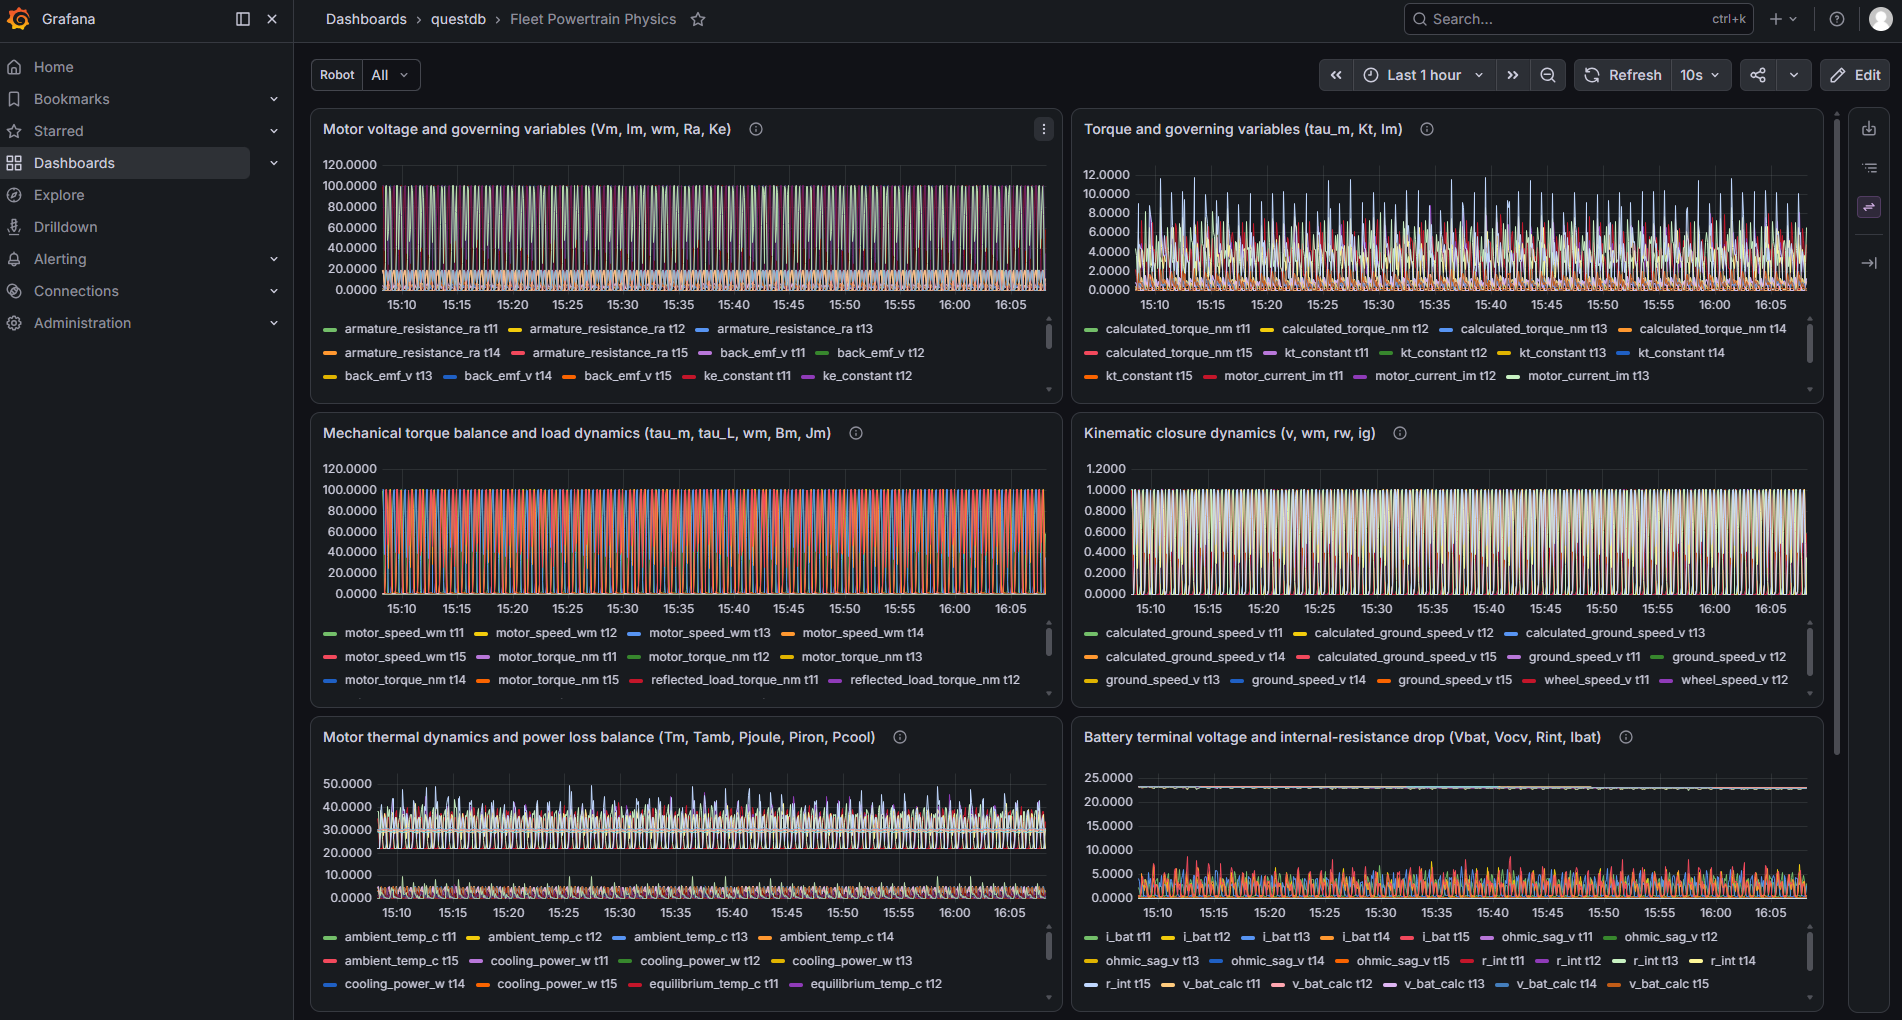
\includegraphics[width=0.95\linewidth]{grafanaFleetPowertrainPhysicsDashboard.png}
  \caption{Grafana Fleet Powertrain Physics dashboard.}
  \label{fig:manual-grafana-powertrain}
\end{figure}

\begin{figure}[ht]
  \centering
  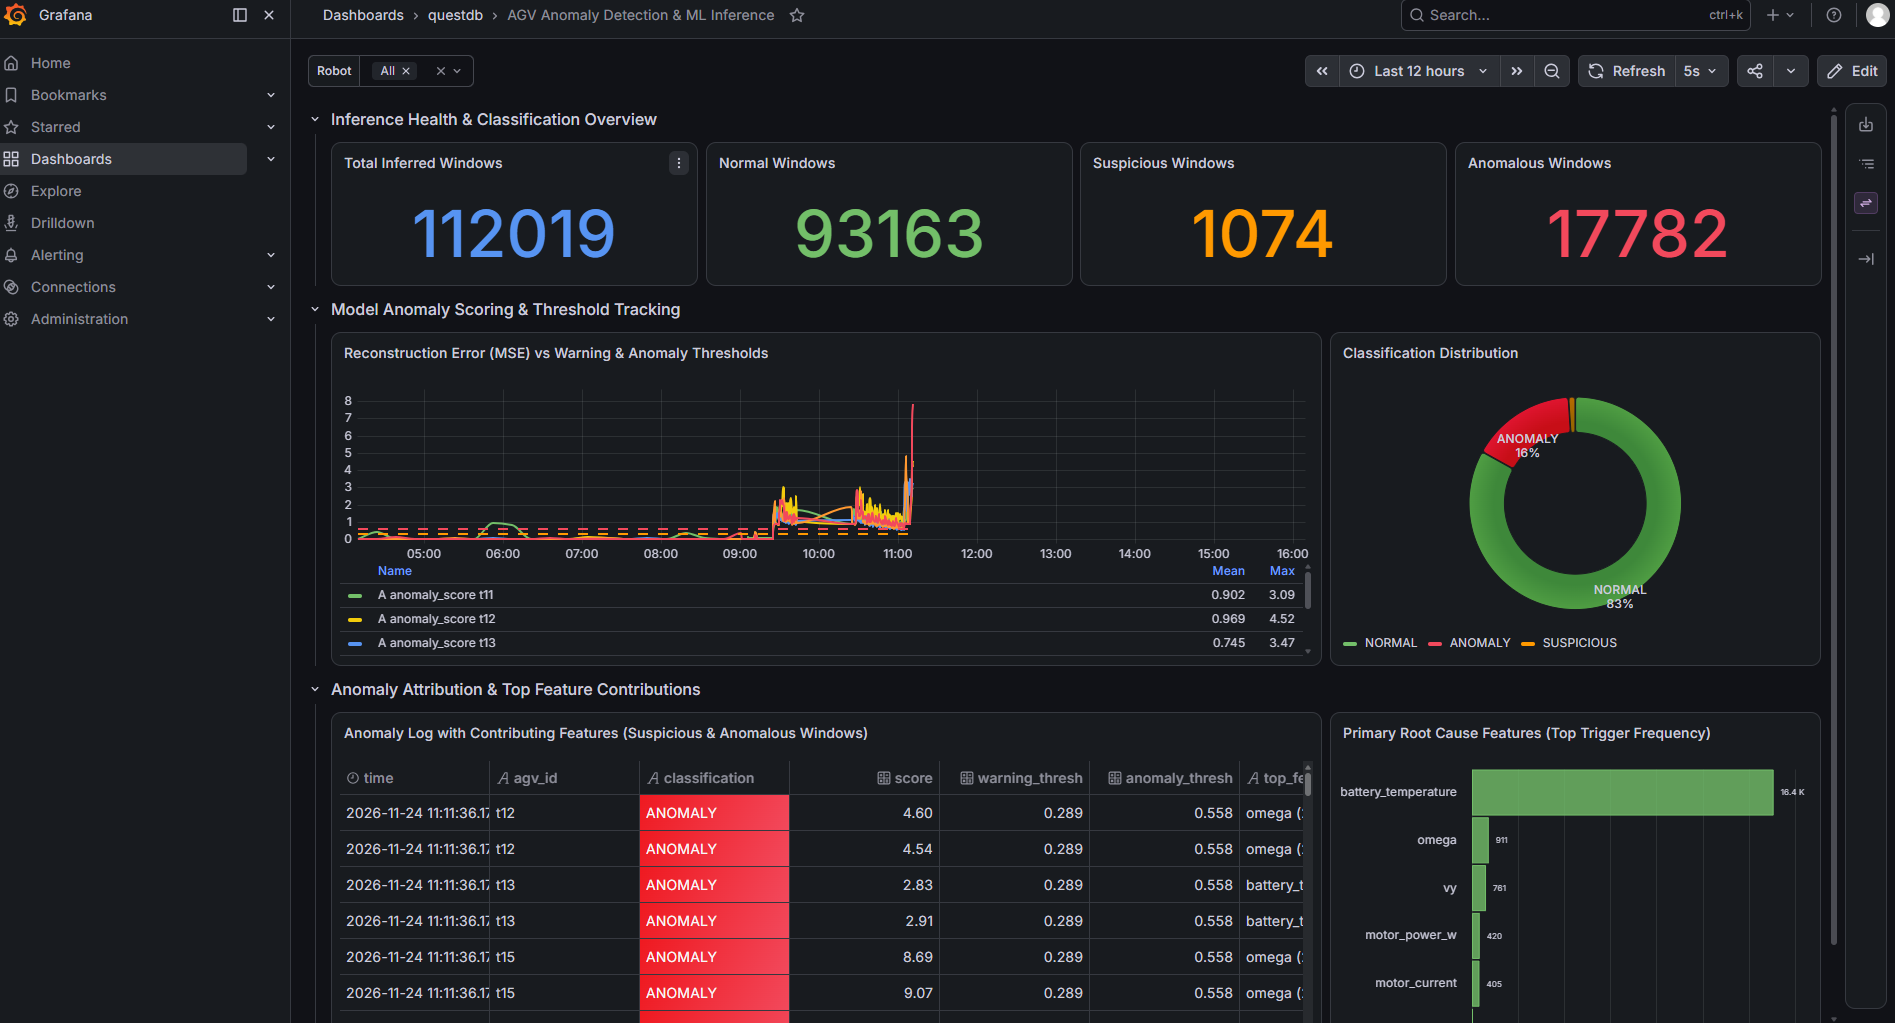
\includegraphics[width=0.95\linewidth]{grafanaMlInterfaceDashboard.png}
  \caption{Grafana anomaly detection dashboard, with the score, the two thresholds, and the class counts.}
  \label{fig:manual-grafana-anomaly}
\end{figure}

The anomaly dashboard stays empty until inference is scoring. Scoring starts when the registry has a version aliased \texttt{production}. Telemetry dashboards do not wait for that alias.

\section{Inspecting the live data}

Redpanda Console at \texttt{http://localhost:9080} shows the three topics. \texttt{vda5050-state} is the raw vehicle state. \texttt{fleet-features} is the curated stream. \texttt{ai-anomalies} is the score stream. Open a topic and read the latest records. The key of a record is the vehicle.

\begin{figure}[ht]
  \centering
  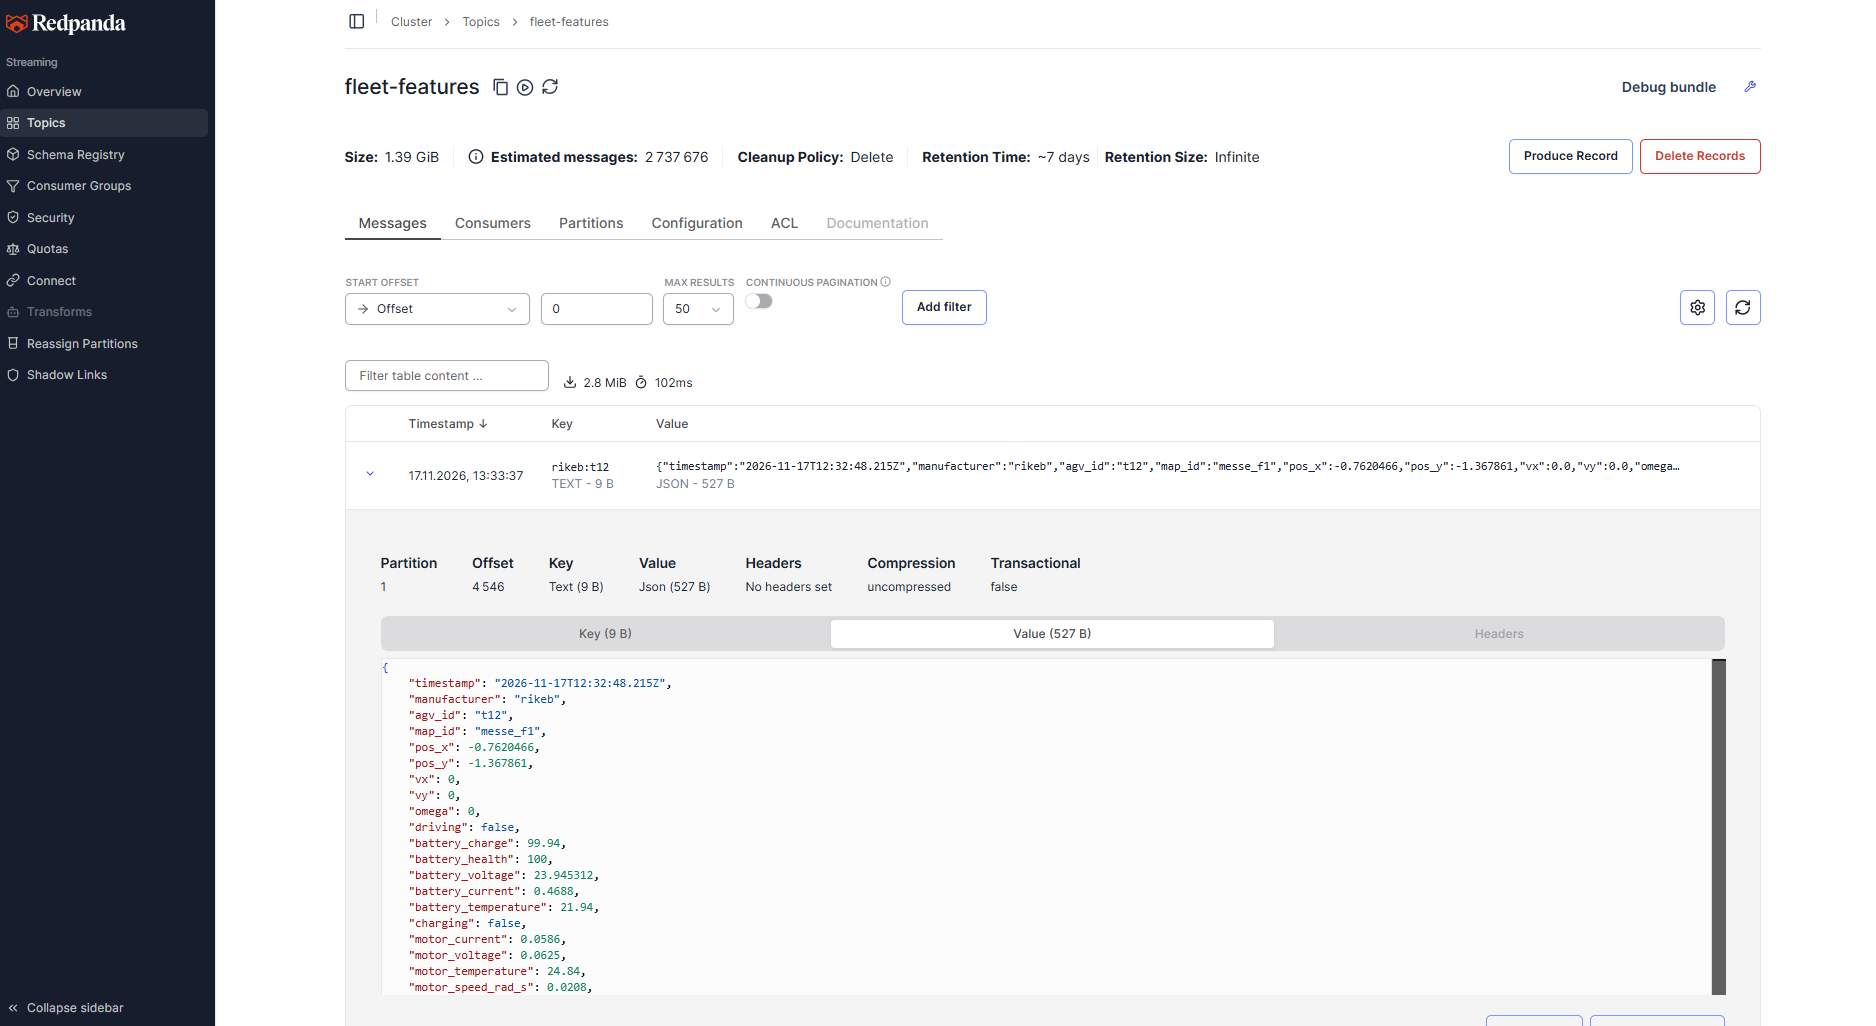
\includegraphics[width=0.95\linewidth]{inspectingTheLiveDataRedpanda.png}
  \caption{Redpanda Console opened on the \texttt{fleet-features} topic.}
  \label{fig:manual-redpanda}
\end{figure}

QuestDB at \texttt{http://localhost:9000} answers SQL against the same operational tables. A recent window of features for one vehicle is:

\begin{lstlisting}[basicstyle=\ttfamily\small,breaklines=true]
SELECT timestamp, agv_id, vx, omega, motor_current, battery_voltage
FROM fleet_features
WHERE agv_id = 't11'
ORDER BY timestamp DESC
LIMIT 20;
\end{lstlisting}

The anomaly table is \texttt{ai\_anomalies}. The columns to read first are \texttt{anomaly\_score}, \texttt{classification} (\texttt{NORMAL}, \texttt{SUSPICIOUS}, \texttt{ANOMALY}), and the top-feature fields.

\begin{figure}[ht]
  \centering
  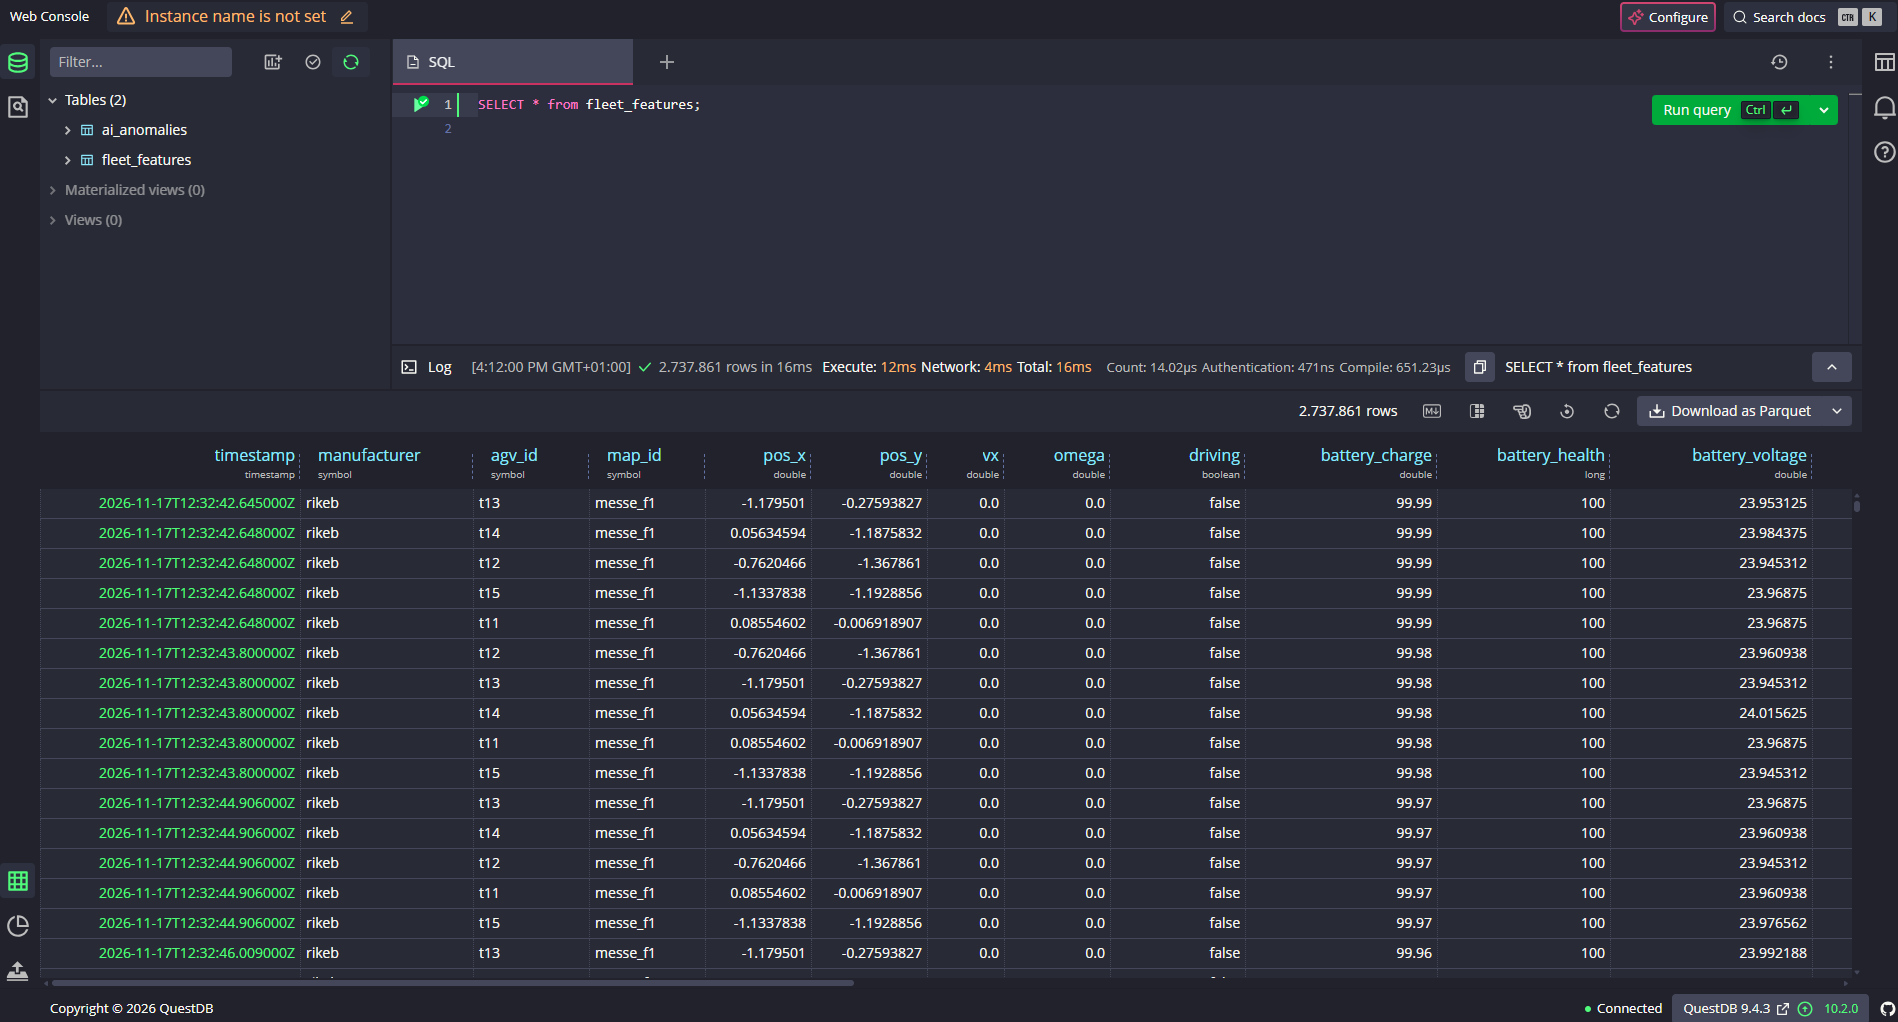
\includegraphics[width=0.95\linewidth]{inspectingTheLiveDataQuestDB.png}
  \caption{QuestDB console with a query on \texttt{fleet\_features}.}
  \label{fig:manual-questdb}
\end{figure}

MinIO at \texttt{http://localhost:9001} (\texttt{admin} / \texttt{admin123456}) shows the \texttt{lakehouse} bucket. The Bronze and Silver Parquet files live there. Day-to-day reading of telemetry is easier in QuestDB. MinIO is the place to confirm that the lakehouse is receiving files.

\section{Promoting a model}

After the training command in Appendix~\ref{app:installation_manual}, open MLflow at \texttt{http://localhost:5000}. The run sits in the experiment \texttt{agv-anomaly-detection}. Its name has the form \texttt{gru-h64-l32-w60-} followed by the dataset label. The comparable column is \texttt{val/loss\_best}.

Registering the network creates a new version of \texttt{agv-gru-autoencoder}. Inference does not load a version merely because it is the latest. Figure~\ref{fig:manual-promote} shows the registry after a demonstration version was added: version~6 carries the manual label and has no alias, and version~5 keeps \texttt{production}. The stream continues to serve version~5. To promote a later model, set that alias on the version that should be served. Within about a minute the inference job adopts that version and its scaler together. The anomaly dashboard then starts to fill.

\begin{figure}[ht]
  \centering
  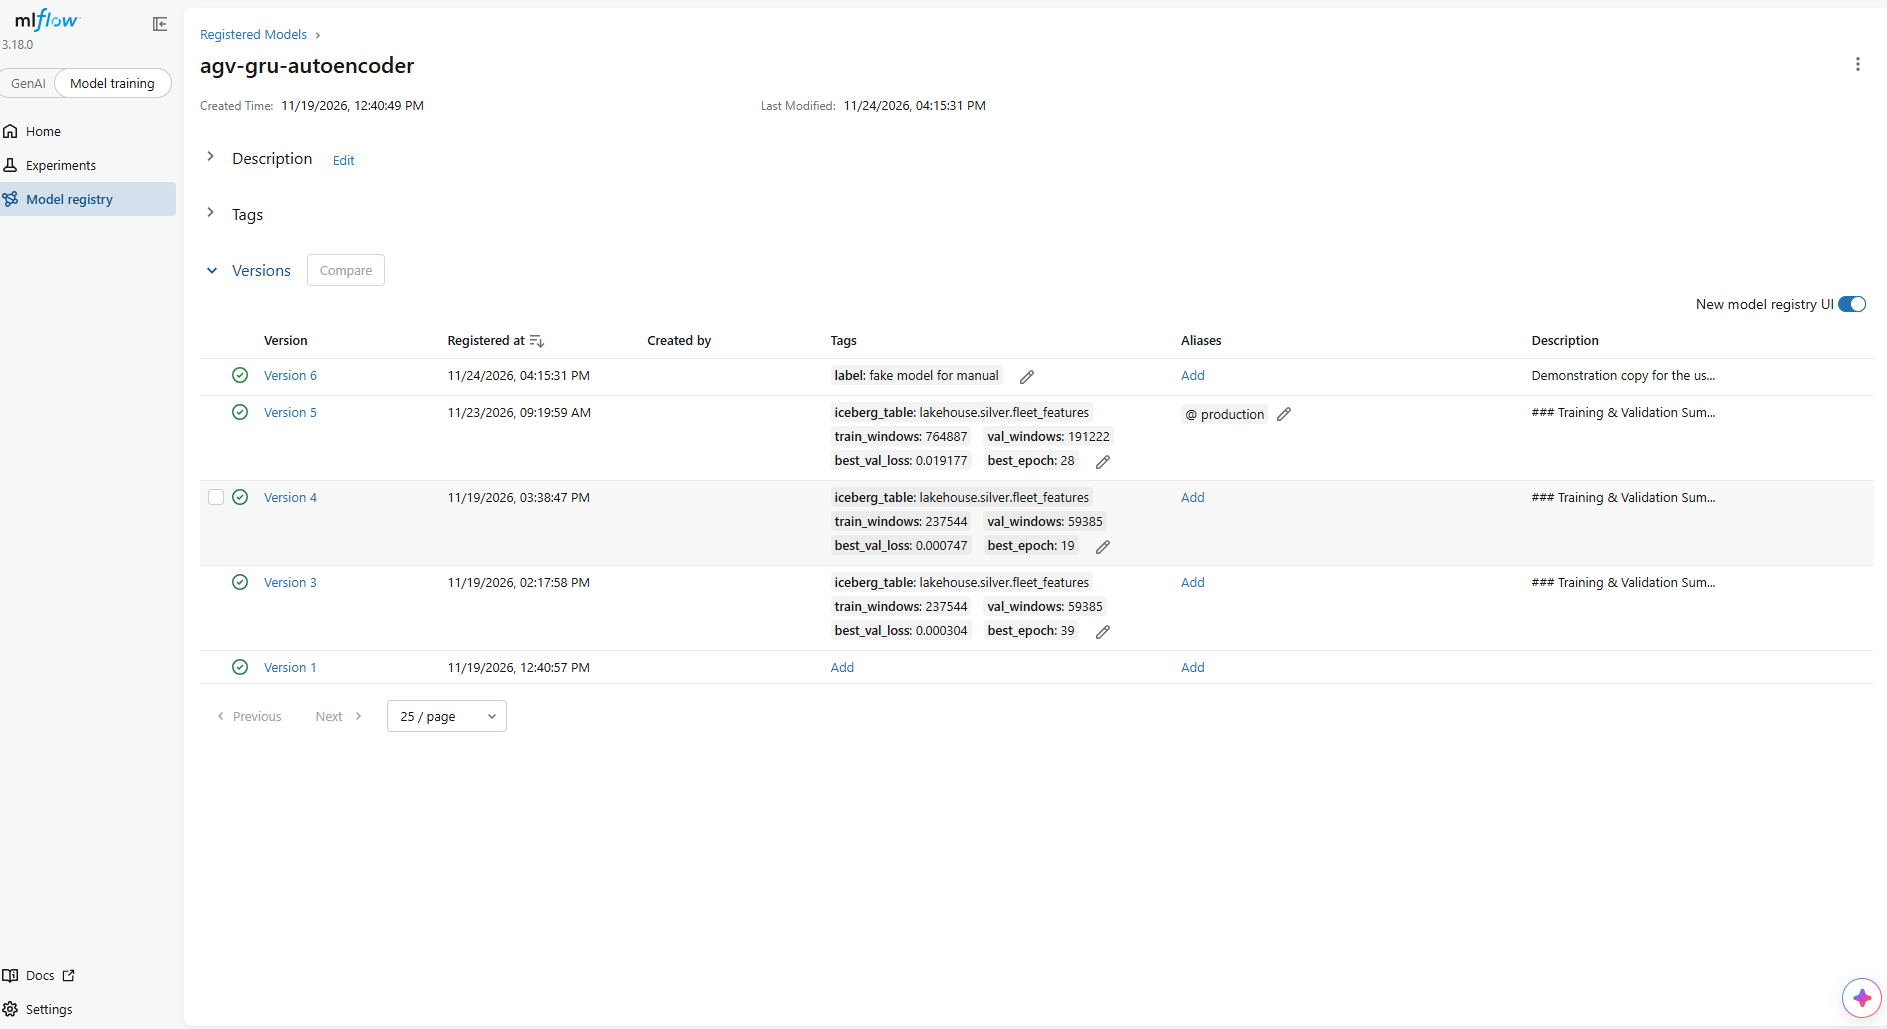
\includegraphics[width=0.95\linewidth]{promotingAModel.png}
  \caption{Model registry for \texttt{agv-gru-autoencoder}. Version~6 is the demonstration copy and has no alias. Version~5 keeps the \texttt{production} alias.}
  \label{fig:manual-promote}
\end{figure}

% !TeX root = ../main.tex
\chapter{Deployment Manifests and Simulator Specification}
\label{app:deployment}

This appendix collects the deployment files, the Telegraf bridge configuration, the QuestDB table definitions, and the specification used to extend the vehicle simulator. Chapter~\ref{chap:system_implementation} describes what those files do. The listings are the files of the prototype, copied so the manuscript can be read without the repository open beside it. Credentials in them are the local development defaults.

\section{Docker Compose}
\label{sec:app_compose}

The root file includes one Compose file per subsystem, declares the bridge networks, and mounts the partner certificate. The simulator include also applies the override that builds the image from source. Telegraf is the telemetry-bridge file: it is no longer a service of the MQTT broker. Training is the \texttt{ml} profile of the machine-learning module and does not start with \texttt{docker compose up}.

\lstinputlisting[language=yaml,caption={Root Compose file},label={lst:main-compose},basicstyle=\ttfamily\footnotesize,breaklines=true]{appendices/compose/root.yml}

\lstinputlisting[language=yaml,caption={MQTT broker},label={lst:mqtt-broker-compose},basicstyle=\ttfamily\footnotesize,breaklines=true]{appendices/compose/mqtt-broker.yml}

\lstinputlisting[language=yaml,caption={Vehicle simulator},label={lst:vda5050-simulator-docker-compose},basicstyle=\ttfamily\footnotesize,breaklines=true]{appendices/compose/simulator.yml}

\lstinputlisting[language=yaml,caption={Simulator build override},label={lst:simulator-override},basicstyle=\ttfamily\footnotesize,breaklines=true]{appendices/compose/simulator-override.yml}

\lstinputlisting[language=yaml,caption={Redpanda},label={lst:redpanda-docker-compose},basicstyle=\ttfamily\footnotesize,breaklines=true]{appendices/compose/redpanda.yml}

\lstinputlisting[language=yaml,caption={Spark streaming jobs},label={lst:spark-docker-compose},basicstyle=\ttfamily\footnotesize,breaklines=true]{appendices/compose/spark.yml}

\lstinputlisting[language=yaml,caption={MinIO},label={lst:minio-docker-compose},basicstyle=\ttfamily\footnotesize,breaklines=true]{appendices/compose/minio.yml}

\lstinputlisting[language=yaml,caption={Telemetry bridge},label={lst:telemetry-bridge-compose},basicstyle=\ttfamily\footnotesize,breaklines=true]{appendices/compose/telemetry-bridge.yml}

\lstinputlisting[language=yaml,caption={QuestDB},label={lst:questdb-compose},basicstyle=\ttfamily\footnotesize,breaklines=true]{appendices/compose/questdb.yml}

\lstinputlisting[language=yaml,caption={Grafana},label={lst:grafana-compose},basicstyle=\ttfamily\footnotesize,breaklines=true]{appendices/compose/grafana.yml}

\lstinputlisting[language=yaml,caption={MLflow},label={lst:mlflow-compose},basicstyle=\ttfamily\footnotesize,breaklines=true]{appendices/compose/mlflow.yml}

\lstinputlisting[language=yaml,caption={Training module},label={lst:ml-module-compose},basicstyle=\ttfamily\footnotesize,breaklines=true]{appendices/compose/ml-module.yml}

\lstinputlisting[language=yaml,caption={Factory orchestrator},label={lst:orchestrator-compose},basicstyle=\ttfamily\footnotesize,breaklines=true]{appendices/compose/factory-orchestrator.yml}

\lstinputlisting[language=yaml,caption={Digital twin},label={lst:twin-compose},basicstyle=\ttfamily\footnotesize,breaklines=true]{appendices/compose/digital-twin.yml}

\lstinputlisting[language=yaml,caption={Platform portal},label={lst:portal-compose},basicstyle=\ttfamily\footnotesize,breaklines=true]{appendices/compose/platform-portal.yml}

\section{Telegraf configuration}
\label{sec:app_telegraf}

The bridge in Section~\ref{subsec:telegraf_integration} is configured by this file. It is mounted into the Telegraf service of Listing~\ref{lst:telemetry-bridge-compose}.

\lstinputlisting[language=configToml,caption={Telegraf bridging configuration (telegraf.conf)},label={lst:telegraf-conf},basicstyle=\ttfamily\footnotesize,breaklines=true]{appendices/config/telegraf.conf}

\section{QuestDB tables}
\label{sec:app_questdb_schema}

\texttt{questdb-init} applies these two files, as described in Section~\ref{subsec:questdb-deployment-schema}.

\lstinputlisting[language=SQL,caption={QuestDB table \texttt{fleet\_features}},label={lst:fleet-features-sql},basicstyle=\ttfamily\footnotesize,breaklines=true]{appendices/schema/fleet_features.sql}

\lstinputlisting[language=SQL,caption={QuestDB table \texttt{fleet\_anomalies}},label={lst:fleet-anomalies-sql},basicstyle=\ttfamily\footnotesize,breaklines=true]{appendices/schema/fleet_anomalies.sql}

\section{Specification used to extend the simulator}
\label{app:simulator_prompt}

The electromechanical extension of the simulator was specified to the model as the document below, and the generated code was reviewed against it before it was kept. The first draft asked for a separate physics task, a full armature inductance, a polarisation branch in the battery, and a stator short. The integrated simulator does not do those, and it adds wheel wear as a drop in rolling resistance, bearing wear, a housing-vibration RMS, the accelerated discharge, and the depletion stop. Those departures are marked in the document as implemented deviations, so the text matches the simulator that publishes the telemetry. The equations used in Chapter~\ref{chap:system_implementation} are the ones this specification settles on.

\lstinputlisting[caption={Simulator extension specification},label={lst:simulator-prompt},basicstyle=\ttfamily\footnotesize,breaklines=true]{appendices/prompt/complete_sensor_adaptation.md}

